\begin{exercise}
      {ID-c62dbe547d605460bea3082d3d4523f52cfa69cd}
      {15 Grad}
  \ifproblem\problem\par
    Innerhalb eines Quadrats liegt ein Punkt $M$, für den $\measuredangle
    BAM=\measuredangle MBA=15^{\circ}$ Basiswinkel eines gleichschenkligen
    Dreiecks sind. Wie groß ist dann der Winkel $\measuredangle CMD$?
    \begin{center}
      \begin{tikzpicture}
        \coordinate (A) at (0, 0);
        \coordinate (B) at (3, 0);
        \coordinate (C) at (3, 3);
        \coordinate (D) at (0, 3);
        \coordinate (A2) at ([shift={(15:3)}]A);
        \coordinate (B2) at ([shift={(165:3)}]B);
        \coordinate (M)  at (intersection of A--A2 and B--B2);
        \fill (A) circle[radius=1pt] node[below left]  {$A$};
        \fill (B) circle[radius=1pt] node[below right] {$B$};
        \fill (C) circle[radius=1pt] node[above right] {$C$};
        \fill (D) circle[radius=1pt] node[above left]  {$D$};
        \fill (M) circle[radius=1pt] node[above]       {$M$};
        \draw (A) -- (B) -- (C) -- (D) -- cycle;
        \draw (A) -- (M) -- (B);
      \end{tikzpicture}
    \end{center}
  \fi
  \ifoutline\outline\par
    Benutze den \emph{Tangens}, um $\alpha$ zu bestimmen.
    \begin{center}
      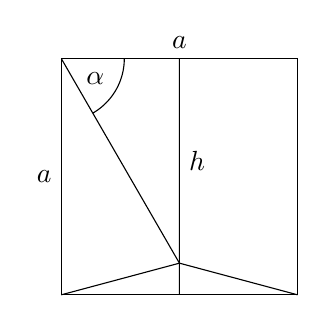
\begin{tikzpicture}
        \coordinate (A) at (0, 0);
        \coordinate (B) at (3, 0);
        \coordinate (C) at (3, 3);
        \coordinate (D) at (0, 3);
        \coordinate (A2) at ([shift={(15:3)}]A);
        \coordinate (B2) at ([shift={(165:3)}]B);
        \coordinate (M)  at (intersection of A--A2 and B--B2);
        \draw (A) -- (B) -- (C) -- (D) -- cycle;
        \draw (A) -- (M) -- (B);
        \draw (D) -- (M);
        \draw (M) -- (1.5, 0);
        \draw (1.5, 3) -- node[right]{$h$} (M);
        \node[left]  at (0, 1.5) {$a$};
        \node[above] at (1.5, 3) {$a$};
        \begin{scope}
          \clip (M) -- (1.5, 3) -- (D) -- cycle;
          \draw (D) circle[radius=8mm];
          \node at ([shift={(330:5mm)}]D) {$\alpha$};
        \end{scope}
      \end{tikzpicture}
    \end{center}
  \fi
  \ifoutcome\outcome\par
    \begin{minipage}{5cm}
      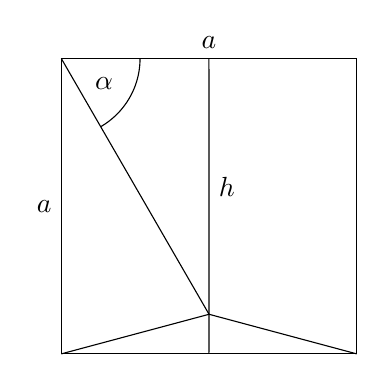
\begin{tikzpicture}[scale=1.25]
        \coordinate (A) at (0, 0);
        \coordinate (B) at (3, 0);
        \coordinate (C) at (3, 3);
        \coordinate (D) at (0, 3);
        \coordinate (A2) at ([shift={(15:3)}]A);
        \coordinate (B2) at ([shift={(165:3)}]B);
        \coordinate (M)  at (intersection of A--A2 and B--B2);
        \draw (A) -- (B) -- (C) -- (D) -- cycle;
        \draw (A) -- (M) -- (B);
        \draw (D) -- (M);
        \draw (M) -- (1.5, 0);
        \draw (1.5, 3) -- node[right]{$h$} (M);
        \node[left]  at (0, 1.5) {$a$};
        \node[above] at (1.5, 3) {$a$};
        \begin{scope}
          \clip (M) -- (1.5, 3) -- (D) -- cycle;
          \draw (D) circle[radius=8mm];
          \node at ([shift={(330:5mm)}]D) {$\alpha$};
        \end{scope}
      \end{tikzpicture}
    \end{minipage}%
    \begin{minipage}{9cm}
      \begin{equation*}
        \begin{split}
          \tan(15^{\circ})&=\frac{a-h}{\frac{a}{2}}
                    \quad\Rightarrow\quad
                    h=a-\frac{a}{2}\cdot\tan(15^{\circ})\\[2ex]
          \tan(\alpha)&=\frac{h}{\;\frac{a}{2}\;}
                       =\frac{a-\frac{a}{2}\cdot\tan(15^{\circ})}{\frac{a}{2}}\\[2ex]
                      &=2-\tan(15^{\circ})
                       =2-(2-\sqrt{3})=\sqrt{3}\\[3ex]
          \Rightarrow\quad\alpha&=\arctan(\sqrt{3})=60^{\circ}
        \end{split}
      \end{equation*}
    \end{minipage}\bigskip\par
    Damit sind die beiden Basiswinkel $\alpha$ des oberen Dreiecks $60^{\circ}$,
    und wegen der konstanten Innenwinkelsumme von $180^{\circ}$ in Dreiecken
    der gesuchte dritte Winkel auch. Das Dreieck $\triangle MCD$ ist also gleichseitig.
  \fi
\end{exercise}
